\subsection{Homotopy Continuation}
\label{sec:homotopy}

Homotopy continuation~\cite{HomotophyContinuationMethods} is a powerful numerical–symbolic method for solving systems of nonlinear (especially polynomial) equations by deforming a solvable start system into the target system and tracking solution paths continuously.

More formally, given \(F(x)=0\) to solve where \(x\in\mathbb{C}^n\), we construct a homotopy
\begin{align}
H(x,t) = (1-t)\,G(x) + t\,F(x), \\ H(x,0)=G(x),\, \; H(x,1)=F(x),
\end{align}
where \(G\) has known regular solutions.

Algorithm~\ref{alg:homotopy_path_tracking} summarizes an Homotopy continuation iter.
Starting from a known solution \(x(0)\) (line 2), we numerically follow the curve \(x(t)\) satisfying \(H(x(t), t)=0\) from $t=0$ to $t=1$ (line 3).
Using the differential notation we can write
\[
\frac{\partial H}{\partial x} \dot x + \frac{\partial H}{\partial t} = 0 \quad\Rightarrow\quad \dot x = -\left(\frac{\partial H}{\partial x}\right)^{-1} \frac{\partial H}{\partial t},
\]
to find out the direction of the solution path at each step. That can be solved using any ODE method, such as Euler's method or Runge-Kutta methods (line 4).
We compute the new value of \(x\) at \(t+\Delta t\) by using a predictor step (line 5).
Then we correct the prediction using Newton’s method making it consistent with \(H(x, t+\Delta t)=0\) (line 7).
We then iterate the process until we reach $t=1$.

\begin{figure}[H]
	\centering
	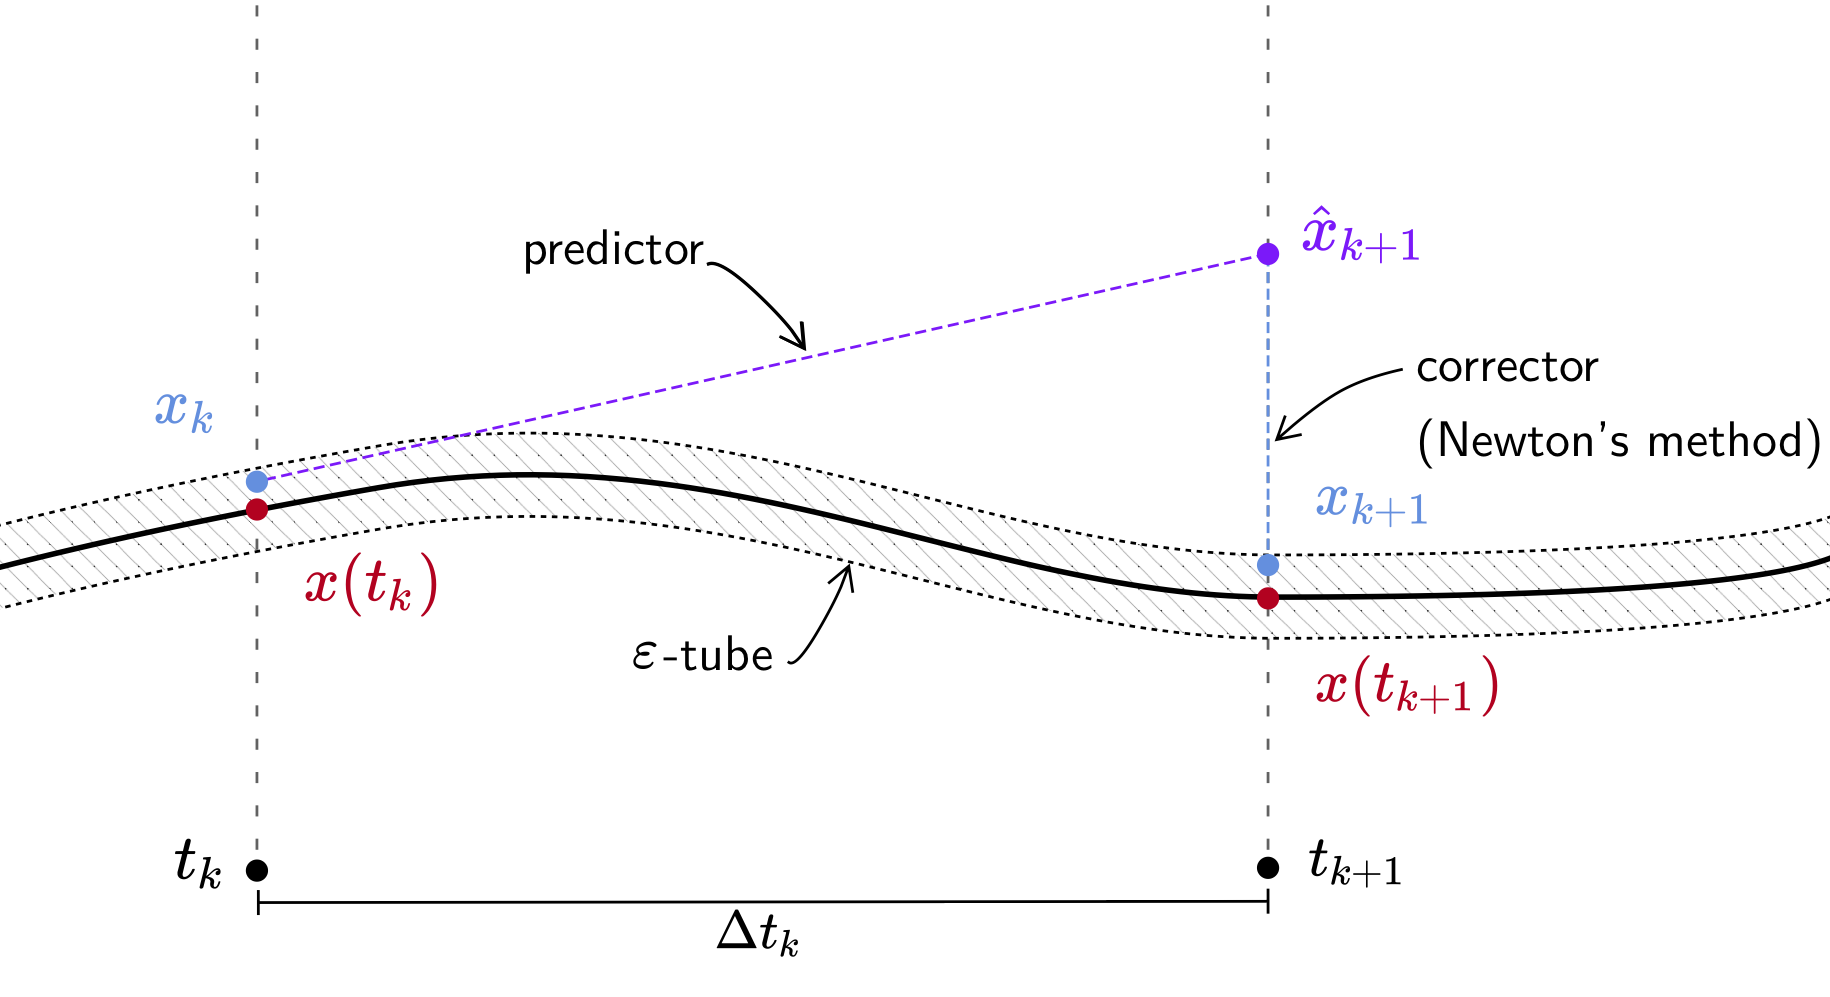
\includegraphics[width=0.85\linewidth]{images/homotopy_predictor_corrector}
	\caption{A sketch of the predictor-corrector method. We compute a prediction $\tilde x = x_k + \Delta t\,\dot x_k$ using any ODE method and then correct using Newton's method.}
	\label{fig:homotopy_predictor_corrector}
\end{figure}

% Algorithm: Homotopy Path Tracking (Predictor-Corrector Loop)
\begin{algorithm}[H]
\caption{Homotopy Path Tracking via Predictor-Corrector}
\label{alg:homotopy_path_tracking}
\begin{algorithmic}[1]
\REQUIRE Initial solution $x_0$, initial time $t_0 = 0$, step size $\Delta t$
\STATE $k \leftarrow 0$
\STATE $x_k \leftarrow x_0$, $t_k \leftarrow t_0$
\WHILE{$t_k < 1$}
    \STATE Compute $\dot x_k = -\left(\frac{\partial H}{\partial x}(x_k, t_k)\right)^{-1} \frac{\partial H}{\partial t}(x_k, t_k)$
    \STATE $\tilde x \leftarrow x_k + \Delta t\,\dot x_k$ \; (Predictor: Euler or higher order)
    \STATE $t_{k+1} \leftarrow t_k + \Delta t$
    \STATE $x_{k+1} \leftarrow$ Newton's method to solve $H(x, t_{k+1})=0$ starting from $\tilde x$
    \STATE $k \leftarrow k+1$
\ENDWHILE
\RETURN $x_k$ (approximate solution to $F(x)=0$)
\end{algorithmic}
\end{algorithm}

\subsection {Parametric Homotopy}
\label{sec:parametric_homotopy}
In many applications, a polynomial system can be seen as a specific instance (Figure~\ref{fig:monodromy_original}) of a family of polynomial systems that depend on parameters.
For example, consider the insersections of two parabolae curves, which can be described by the polynomial system
\[
F(x; p) = \begin{pmatrix}
p_1 x^2 + p_2 x + p_3 - y = 0 \\
p_4 x^2 + p_5 x + p_6 - y = 0
\end{pmatrix},
\]
where \(p = (p_1, p_2, p_3, p_4, p_5, p_6)\) are the parameters that define the specific instance of the system. Changing the parameters \(p\) will change the shape and position of the curves, thus changing the solution set of the system \(F(x; p) = 0\). The solution set will vary continuously as the parameters change, and we can track how the solutions evolve as we vary \(p\). By just varying the parameters, we can explore a vast range of solutions from two points intersections, one tangent point, to no intersections at all.

\begin{figure}[hb]
	\centering
	\subfloat[
		A parabola instance of the family $y = p_1 x^2 + p_3$.
	]{
		% 
\includegraphics[width=0.23\linewidth]{images/parametric_homotopy/original}
		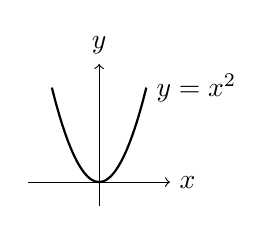
\begin{tikzpicture}[scale=0.3]
			% Draw axes
			\draw[->] (-3, 0) -- (3, 0) node[right] {$x$};
			\draw[->] (0, -1) -- (0, 5) node[above] {$y$};

			% Draw parabola y = x^2
			\draw[domain=-2:2, smooth, variable=\x, black, thick] 
				plot ({\x}, {\x*\x}) node[right] {$y = x^2$};
		\end{tikzpicture}
		\label{fig:parametric_homotopy_original}
	}
	\hspace{0.01\linewidth}
	\subfloat[
		The surface resulting from varying the parameter $p_3$. We can see that the solution set (highlighted in blue) varies continuously as the parameter (Y axis) changes.
	]{
		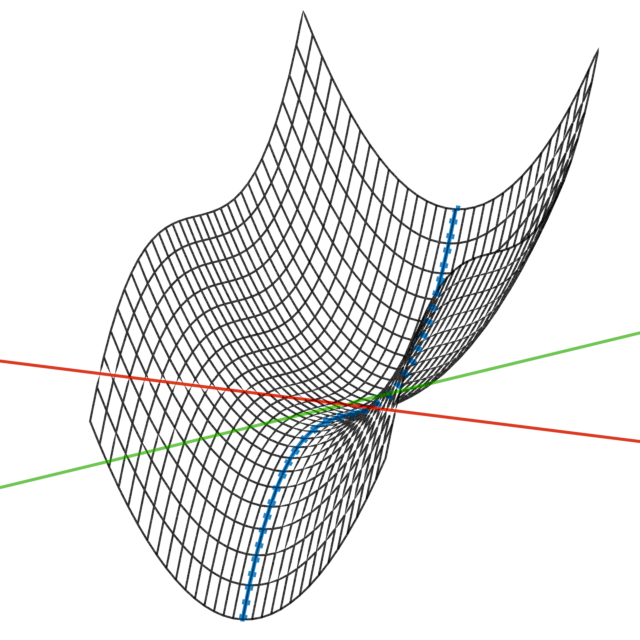
\includegraphics[width=0.23\linewidth]{images/parametric_homotopy/family_surface.png}
		\label{fig:parametric_homotopy_family}
	}
	\hspace{0.01\linewidth}
	\subfloat[
		An instance of the polynomial system $F(x; p) = 0$ with $p = (1, 0, 0, -1, 0, 0)$.
	]{
		% 
\includegraphics[width=0.23\linewidth]{images/parametric_homotopy/instance1}
		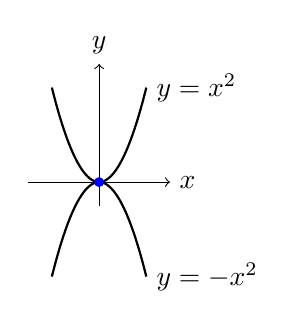
\begin{tikzpicture}[scale=0.3]
			% Draw axes
			\draw[->] (-3, 0) -- (3, 0) node[right] {$x$};
			\draw[->] (0, -1) -- (0, 5) node[above] {$y$};

			% Draw parabola y = x^2
			\draw[domain=-2:2, smooth, variable=\x, black, thick] 
				plot ({\x}, {\x*\x}) node[right] {$y = x^2$};
			% Draw parabola y = -x^2
			\draw[domain=-2:2, smooth, variable=\x, black, thick] 
				plot ({\x}, {-\x*\x}) node[right] {$y = -x^2$};

			% Draw intersection points
			\fill[blue] (0, 0) circle (6pt) node[below right] {};
		\end{tikzpicture}
		\label{fig:parametric_homotopy_instance1}
	}
	\hspace{0.01\linewidth}
	\subfloat[
		An instance of the polynomial system $F(x; p) = 0$ with $p = (1, 0, 1, -1, 0, -1)$.
	]{
		% 
\includegraphics[width=0.23\linewidth]{images/parametric_homotopy/instance2}
		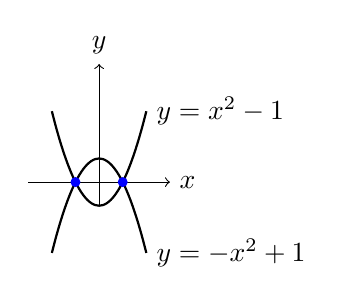
\begin{tikzpicture}[scale=0.3]
			% Draw axes
			\draw[->] (-3, 0) -- (3, 0) node[right] {$x$};
			\draw[->] (0, -1) -- (0, 5) node[above] {$y$};

			% Draw parabola y = x^2 - 1
			\draw[domain=-2:2, smooth, variable=\x, black, thick] 
				plot ({\x}, {\x*\x - 1}) node[right] {$y = x^2 - 1$};
			% Draw parabola y = -x^2 + 1
			\draw[domain=-2:2, smooth, variable=\x, black, thick] 
				plot ({\x}, {-\x*\x + 1}) node[right] {$y = -x^2 + 1$};

			% Draw intersection points
			\fill[blue] (1, 0) circle (6pt) node[below right] {};
			\fill[blue] (-1, 0) circle (6pt) node[below left] {};
		\end{tikzpicture}
		\label{fig:parametric_homotopy_instance2}
	}
	\caption{Parametric homotopy in polynomial systems. The first image shows a parabola instance of the family $y = p_1 x^2 + p_3$, the second shows the surface resulting from varying the parameter $p_3$, and the third and fourth images show two instances of the polynomial system $F(x; p) = 0$ with different parameter values.}
\end{figure}

From such systems we can construct a \emph{parametric homotopy} to track solutions as the parameters vary if for any parameter set $p_0$ a solution $x_0$ is known. In our parabola example, we can take \(p_0 = (1, 0, 0, -1, 0, 0)\) and \(x_0 = (0, 0)\) as a known solution. We can then track solutions as the parameters vary from \(p_0\) to any other parameter set \(p_1\) (e.g., \(p_1 = (1, 0, 0, 1, 0, 1)\)).

More formally, given a polynomial system \(F(x; p) = 0\) where \(x \in \mathbb{C}^n\) are the unknowns, \(p \in \mathbb{C}^m\) are parameters, $p_0$ is a starting parameter set, and $p_1$ is the target parameters set we are interested in, we can construct a homotopy
\[
H(x, p, t) = \,F(x; (1-t)p_0 + tp_1) = 0,
\]
where $p_0$ is a starting set for which we know the solution $x_0$.
We can then track solutions \(x(t; p)\) as \(t\) varies from \(0\) to \(1\) and \(p\) varies over a path in parameter space from $p_0$ to $p_1$.

\subsection{Monodromy}
\label{sec:monodromy}

In the context of polynomial system solving, \emph{monodromy} refers to a technique that exploits the algebraic structure of solution sets by tracking solutions permutations under continuous deformations of the parameters. In particular, when a parameterized polynomial system admits multiple solutions for generic parameter values, monodromy allows us to expand the solution set by performing loops in parameter space. It does so by observing the behaviour of the system when it "runs around" a singularity.

Consider a family of polynomial systems
\[
F(x; p) = 0,
\]
where \( x \in \mathbb{C}^n \) are the unknowns and \( p \in \mathbb{C}^m \) are parameters. Given at least one solution \( x_0 \) corresponding to a parameter value \( p_0 \) (Figure~\ref{fig:monodromy_original}), we project it into the surface defined by all possible parametrization~\ref{fig:monodromy_parameter_surface}, we construct a path in parameter space that starts and ends at \( p_0 \) (Figure~\ref{fig:monodromy_midloop}). By numerically tracking the solution \( x_0 \) along this loop (via homotopy continuation), we obtain a solution \( x_1 \) at \( p_0 \). In general, \( x_1 \) may differ from \( x_0 \), having traversed a different branch of the solution variety. Repeating this process along different loops allows the discovery of new solutions without prior knowledge of the entire solution set (Figure~\ref{fig:monodromy_conclusive}).

This method relies on the fact that the solution set over generic parameters forms a branched covering of parameter space, and monodromy paths induce permutations (forming the so-called \emph{monodromy group}) on the fiber of solutions above a generic parameter value. Under mild assumptions, if the monodromy group is transitive, sufficiently many loops will recover all solutions.

Monodromy methods serve as a valuable complement to classical homotopy continuation, especially when computing all solutions via total-degree or multihomogeneous start systems is computationally prohibitive.

For additional details on practical implementations, we refer to the monodromy functionality in \texttt{HomotopyContinuation.jl}~\cite{HomotopyContinuationJL}.

\begin{figure}[hb]
	\centering
	\subfloat[Instance of a realization of the polynomial system family $F(x; p) = 0$.]{
		\begin{tikzpicture}
			\node[anchor=south west, inner sep=0] (image) at (0,0) {
\includegraphics[width=0.21\linewidth]{monodromy/original.png}};
			\begin{scope}[x={(image.south east)}, y={(image.north west)}]
				\node at (0.5, 0.17) {$F(x; p_0)$};
				\node at (0.5,0.47) {$x_0$};
			\end{scope}
		\end{tikzpicture}
		\label{fig:monodromy_original}
	}
	\hspace{0.01\linewidth}
	\subfloat[Polynomial system family $F(x; p) = 0$ surface for different values of $p$]{
		\begin{tikzpicture}
			\node[anchor=south west, inner sep=0] (image) at (0,0) {
\includegraphics[width=0.21\linewidth]{monodromy/parameter_surface.png}};
			\begin{scope}[x={(image.south east)}, y={(image.north west)}]
				\node at (0.5, 0.17) {$F(x; p)$};
			\end{scope}
		\end{tikzpicture}
		\label{fig:monodromy_parameter_surface}
	}
	\hspace{0.01\linewidth}
	\subfloat[Mid-loop in parameter space.]{
		
\includegraphics[width=0.21\linewidth]{monodromy/midloop.png}
		\label{fig:monodromy_midloop}
	}
	\hspace{0.01\linewidth}
	\subfloat[Conclusive loop in parameter space. Two new solutions are found.]{
		
\includegraphics[width=0.21\linewidth]{monodromy/successful_monodromy.png}
		\label{fig:monodromy_conclusive}
	}
	\hspace{0.1cm}
	\caption{Monodromy in polynomial system solving. The first image shows a realization of the polynomial system family, the second shows the parameter surface with the known solution $x_0$ highlighted in green. After projecting the surface a circular loop in $x$, $p$ space (highlighted in blue) is constructed (third image). A flat circular loop in this space is not flat on the surface (highlighted in red), so the solution $x_1$ at the end of the loop might not be the same as $x_0$. The fourth image shows a conclusive loop in parameter space that finds two new solutions (highlighted in green).}
	\label{fig:monodromy}
\end{figure}
